\section{DESENVOLVIMENTO}
    \subsection{EXPOSIÇÃO DO TEMA OU MATÉRIA}
    \subsubsection{Formatação do texto}
    \paragraph{As ilustrações}

        \noindent A primeira figura é \acrfull{RBC}

        \begin{figure}[htp]
            \centering
            \caption{Capital Market Line}
            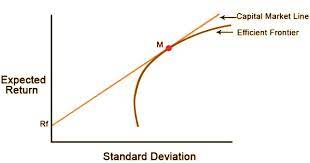
\includegraphics[width=0.5\textwidth]{./imagens/cml.jpg}
            \par \footnotesize Fonte: próprio autor.
            \label{fig:cml}
        \end{figure}


    \paragraph{Equações e fórmulas}
    
    \subparagraph{Exemplo tabela}
        
        \begin{table}[H]
            \centering
            \caption{Tabela inicial do método simplex}
            \begin{tabular}{|c|c|c|c|c|c|c|c|c|}
                \hline
                        & $z$   & $x_1$ & $x_2$ & $s_1$ & $s_2$ & $s_3$ & $s_4$ & $b$   \\ \hline
                $z$     & -1    & -3000 & -1000 & 0     & 0     & 0     & 0     & 0     \\ \hline
                $s_1$   & -     & 1     & 0     & 1     & 0     & 0     & 0     & 6     \\ \hline
                $s_2$   & -     & 0     & 1     & 0     & 1     & 0     & 0     & 12    \\ \hline
                $s_3$   & -     & 1     & 1     & 0     & 0     & 1     & 0     & 16    \\ \hline
                $s_4$   & -     & 1     & $-1/2$& 0     & 0     & 0     & 1     & 2     \\ \hline
            \end{tabular}
            \par \footnotesize Fonte: próprio autor.
            \label{tab:5_4-tabela_inicial}
        \end{table}
    
        e de um quadro \acrshort{IA}:

                    
        \begin{quadro}[H]
            \caption{Restrições do modelo}
            \centering
            \begin{tabular}{|c|c|l|}
                \hline
                TIPO                        & Restrição                                     & Descrição                             \\ \hline
                \multirow{2}{*}{CD}         & \multirow{2}{*}{Capacidade de Expedição}      & O CD possui uma capacidade máxima de  \\
                                            &                                               & expedição de itens em cada turno      \\ 
                \hline
                \multirow{17}{*}{Veículos}  & \multirow{4}{*}{Capacidade de Ocupação}       & Cada tipo de veículo possui           \\
                                            &                                               & uma capacidade máxima de ocupação,    \\
                                            &                                               & e pode transportar carga para         \\
                                            &                                               & atender mais de uma loja              \\   \cline{2-3}
                                            & \multirow{3}{*}{Descanso}                     & A cada 12 horas percorridas,          \\
                                            &                                               & o veículo deve permanecer parado      \\
                                            &                                               & por 12 horas para descanso            \\   \cline{2-3}
                                            & \multirow{4}{*}{Custos}                       & Cada tipo de veículo possui           \\
                                            &                                               & um custo fixo por dia de viagem,      \\
                                            &                                               & e um custo variável aplicado à        \\
                                            &                                               & quilometragem percorrida              \\   \cline{2-3}
                                            &                                               & Cada tipo de veículo possui  \\
                                            &                                               & um tempo fixo de carregamento         \\
                                            & Tempo de Carregamento                         & e descarregamento que pode ser        \\
                                            & /Descarregamento                              & adicionado ao tempo de rota           \\
                                            &                                               & independentemente do número           \\
                                            &                                               & de peças transportado                 \\ 
                \hline
            \end{tabular}
            \label{tab:restricoes}
            \par \footnotesize Fonte: próprio autor.
        \end{quadro}

\section{SEÇÃO}
    
    \noindent citação 1, autor único no fim da frase \cite{Markowitz1952} % (MARKOWITZ, 1952)

    \noindent citação 2, 3 autores no fim da frase \cite{Mansini2014} % (MANSINI; OGRYCZAK; SPERANZA, 2014)

    \noindent citação 3, mais de 3 autores no fim da frase \cite{Vukovic2020} % (VUKOVIC et al., 2020)

    \noindent citação 4, auto único na frase \citeonline{Sharpe1964}. % Sharpe (1964).

    \noindent citação 5, 3 autores na frase \citeonline{Mansini2014}. % Mansini, Ogryczak e Speranza (2014).

    \noindent citação 6, mais de 3 autores na frase \citeonline{Vukovic2020}. % Vukovic et al. (2020).